%!TEX root = ../Technische Dynamik.tex

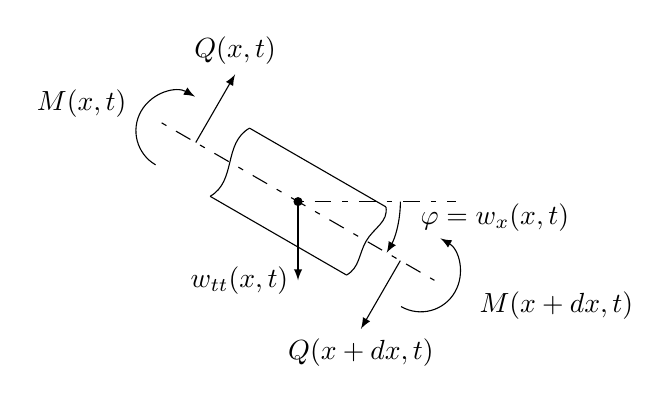
\begin{tikzpicture}[>=latex]
\begin{scope}[rotate=-30]
\draw[dash pattern=on 2pt off 4pt on 6pt off 4pt] (-2,0) -- (2,0);
\draw (-1,-0.5) -- (1,-0.5);
\draw (-1,0.5) -- (1,0.5);
\draw (-1,-0.5) to[in=-120,out=60] (-1,0.5);
\draw (1,-0.5) to[in=-90,out=60] (1,0)  to[in=-50,out=90] (1,0.5);

\draw[->] (-1.5,0) -- (-1.5,1) node[above] {$Q(x,t)$};
\draw[->] (1.5,0) -- (1.5,-1) node[below] {$Q(x+dx,t)$};
\draw[->] (-1.8,-0.5) arc (270:90:0.5);
\node at (-3,-0.3) {$M(x,t)$};
\draw[->] (1.8,-0.5) arc (-90:90:0.5);
\node at (3.5,0.5) {$M(x+dx,t)$};
\end{scope}

\draw[fill] (0,0) circle (0.05);
\draw[->] (0,0) -- (0,-1) node[left] {$w_{tt}(x,t)$};
\draw[dash pattern=on 2pt off 4pt on 6pt off 4pt] (0,0) -- (2,0);

\draw[->] (1.3,0) arc (0:-30:1.3);
\node at (2.5,-0.2) {$\varphi=w_x(x,t)$};
\end{tikzpicture}